\documentclass[final,hyperref={pdfpagelabels=false}]{beamer}
\usepackage[size=custom,orientation=landscape,width=88,7,height=116,2,scale=1.0]{beamerposter}
\usetheme{I6pd2}
\usepackage[utf8]{inputenc}
\usepackage[frenchb]{babel}
\usepackage{amsmath,amsthm,amssymb,latexsym}
\usepackage{times}\usefonttheme{professionalfonts}
\usefonttheme{serif}
\usepackage{booktabs}
\graphicspath{{figures/}}
\usecaptiontemplate{\small\structure{ }\insertcaption}
\usepackage{multicol}
\usepackage{subfigure}
\usepackage{enumitem}
\setbeamercolor{background canvas}{bg=taaluminium,fg=taaluminium}
%%%%%%% TITLE SECTION %%%%%%%
\title{\huge  Object Removal by Exemplar-Based Inpainting \small Based on Criminisi work}
\author{Di Folco Maxime, GIrot Charly, Jallais Maëliss}
\institute{Ecole Supérieure de Chimie Physique Électronique de Lyon}
%%%%%%%% FOOTER %%%%%%%%
%\newcommand{\foot}{* Criminisi et al : Region filling and object removal by exemplar based image inpainting. IEEE Transactions on image processing, 2004 \hfill \break
%*Bertalmio et al, Image Inpainting. Proceedings of the 27th annual conference on Computer graphics and interactive techniques, 2000. }
%\newcommand{\foot}{\textbf{References} : \hfill \break 

\setlist[itemize]{label=$\blacktriangleright$, leftmargin=2cm, font=\normalsize \color{blue}}

\begin{document}
\addtobeamertemplate{block end}{}{\vspace{2ex}}
\begin{frame}[t]

%%%%%%%% INTRODUCTION %%%%%%%%
\begin{columns}[t]
\begin{column}{.02\textwidth} \end{column}
\begin{column}{.930\textwidth} 
\begin{block}{\Large Introduction}

\begin{columns}[t]
\begin{column}{.4\textwidth}
\textbf{Objectif}
\begin{itemize} []
\item \textbf{Supprimer des objets larges} définis par l'utilisateur, à partir d'images numériques
\item Correction d'artefacts ou Restauration d'images
\item Rendu réaliste ou vraisemblable pour l'œil humain
\end{itemize}
\textbf{Principe}
\begin{itemize} 
\item Remplir des régions masquées, par \textbf{propagation de texture} le long des structures linéaires 
\item Utilisation du Principe de \textbf{connectivité} pour définir un ordre de traitement : propager les textures tout en conservant les structures linéaires de l'image
\item Recherche de \textbf{patch similaire} par une analyse couleur
\end{itemize}
\end{column}



\begin{column}{.3\textwidth}

\textbf{État de l'art : 2 grandes approches}
\begin{itemize}
\item Technique d'Inpainting classique [1]
\item Synthèse de textures [?]
\item Mais aussi une combinaison Inpainting/Texture [3]
\end{itemize}

\textbf{Implémentation}
\begin{itemize}
\item Algorithme de \textbf{Criminisi} et al [3]
\item \textbf{OpenCV} C++: gestion des images, des I/O
\item Classes : RegionFill (Algorithmie), Image(I/O), Patch (traitement local)
\end{itemize}

\end{column}

\begin{column}{.29\textwidth}

\begin{figure}[hb] %TO CENTER CAPTION
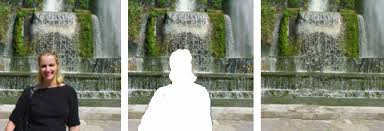
\includegraphics[width=1.0\linewidth]{inpaintingex.jpeg}
\caption{Exemple:  Originale, Suppression de la région, Remplissage de textures }
\label{example}
\end{figure}
\end{column}

\end{columns}
\end{block}
\end{column}


\begin{column}{.02\textwidth} \end{column}
\end{columns}

\begin{columns}[t]

\begin{column}{.02\textwidth} \end{column}

\begin{column}{.465\textwidth} 


\begin{block}{\Large Méthodes}
 
\textbf{Algorithme en 3 étapes principales}
\begin{itemize}
%%%%
\item \textbf{Calcul des priorités} $\forall p \in \delta\Omega P(p)=D(p)C(p) $
\begin{itemize}
\item \textbf{Données} : Quantité de variation des textures autour du pixel courant $D(p) = \dfrac{\mid \nabla I_p^{\perp}.n_p \mid}{\alpha} $
\end{itemize}

\begin{figure}[H]
\centering
\subfigure[Data term itération 0]{\label{fig:data0} 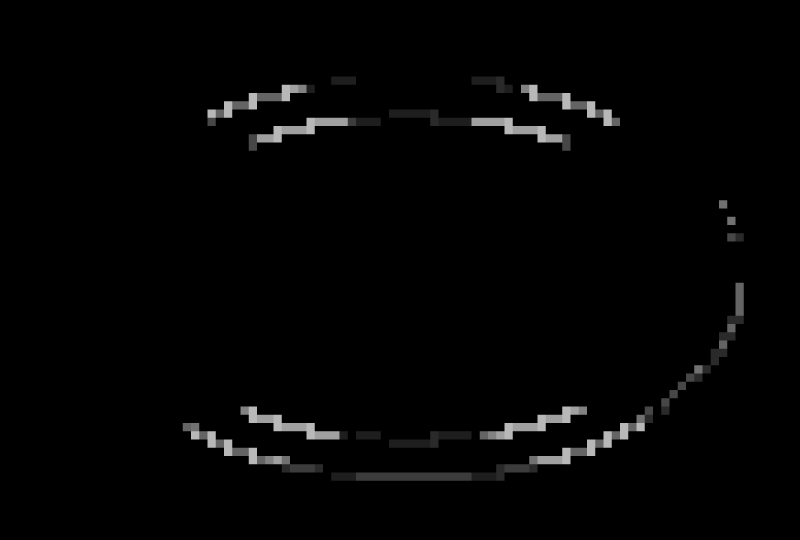
\includegraphics[width=0.3\textwidth]{figures/0data.png}}
\subfigure[data term itération 4]{\label{fig:data1} 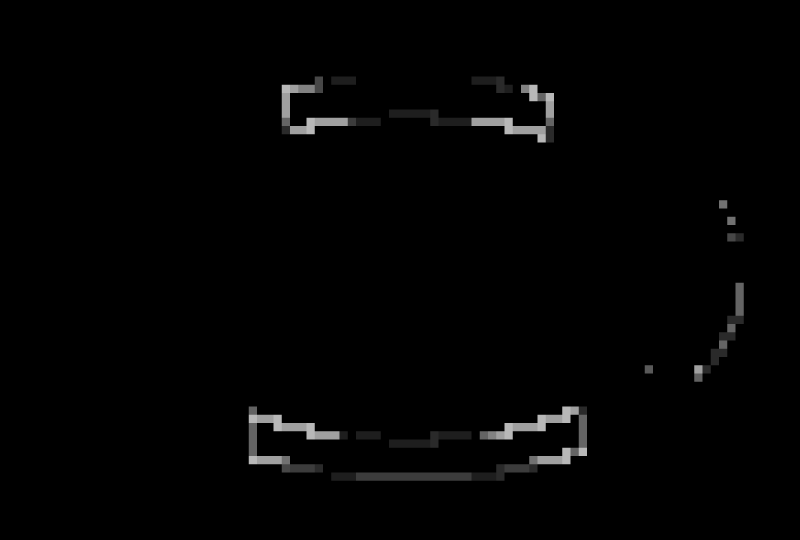
\includegraphics[width=0.3\textwidth]{figures/1data.png}}
\caption{Evolution du terme de données}
\end{figure}

\begin{itemize}
\item \textbf{Confiance} : importance accordée au pixel courant $C(p) = \dfrac{\sum_{q\in \Xi_p \cap(I-\Omega)} C(q)}{\mid \Xi_p\mid} $
\end{itemize}
\begin{figure}[H]
\centering
\subfigure[Confiance itération 0]{\label{fig:kabela} 
\includegraphics[width=0.3\textwidth]{figures/0conf.png}}
\subfigure[Confiance itération 4]{\label{fig:kabelb} 
\includegraphics[width=0.3\textwidth]{figures/1conf.png}}
\caption{Evolution de la confiance}
\end{figure}



%%%\\
%\begin{itemize}
\item \textbf{Propagation de la texture et information structurelle}
\begin{itemize}
\item La priorité est donnée aux \textbf{zones de fortes variations} (terme de données)
\item Propager la texture en commencant par ces zones permet de \textbf{conserver les structures linéaires} de l'image
\item Données de textures manquantes extraites de la zone de l'\textbf{image la plus semblable} (calcul $SSD^a$ dans l'espace couleur Lab)
\end{itemize}

\begin{figure}[H]
\centering
\subfigure[Bordure originale]{\label{fig:priora} 
\includegraphics[width=0.3\textwidth]{figures/0oo.png}}
\subfigure[Bordure après 4 itérations - supprimée là ou la priorité est élevée]{\label{fig:priorb} 
\includegraphics[width=0.3\textwidth]{figures/1oo.png}}
\caption{Evolution de la bordure en fonction de la priorité}
\end{figure}
 
\item \textbf{Mise à jour de la confiance} : Propagation de la confiance du pixel courant vers l'intérieur du masque
\end{itemize}

\end{block}

\end{column}


\begin{column}{.465\textwidth}


\begin{block}{\Large Résultats}

\begin{figure}[H]
\centering
\subfigure[Image Originale]{\label{fig:oval} 
\includegraphics[width=0.4\textwidth]{figures/oval_grand.png}}
\subfigure[Image reconstruite]{\label{fig:ovalb} 
\includegraphics[width=0.4\textwidth]{figures/resultOval51.png}}
\caption{Inpainting d'une image présentant une occlusion}
\end{figure}

\begin{figure}[H]
\centering
\subfigure[Photo Originale]{\label{fig:lincoln} 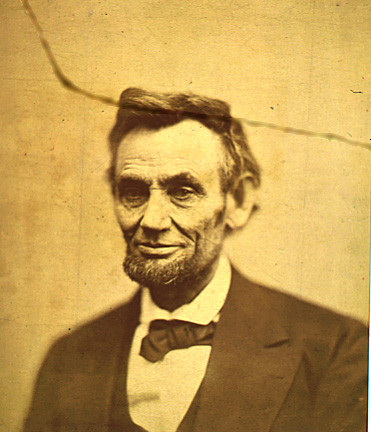
\includegraphics[width=0.4\textwidth]{figures/lincoln.jpg}}
\subfigure[Photo restaurée]{\label{fig:lincolnb} 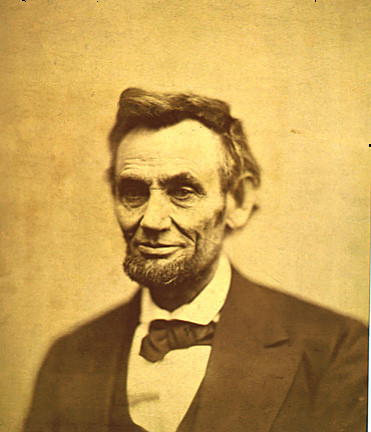
\includegraphics[width=0.4\textwidth]{figures/resultLinc5.png}}
\caption{Restauration d'une image abimée}
\end{figure}
%\begin{figure}[H]
%\centering
%\subfigure[Photo Originale]{\label{fig:troll} 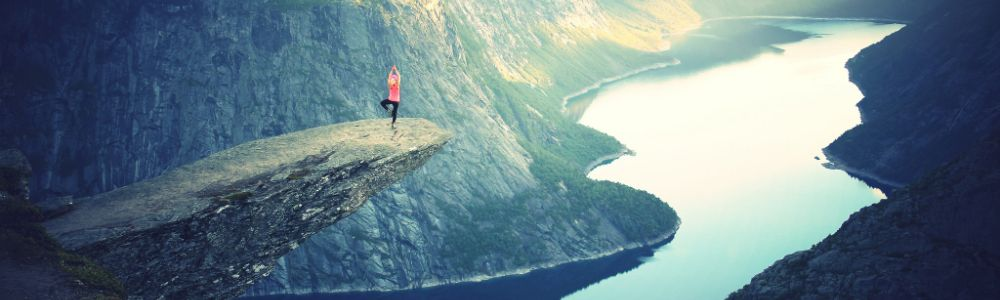
\includegraphics[width=0.4\textwidth]{figures/trolltunga.jpg}}
%\subfigure[Photo avec élément supprimé]{\label{fig:trollb} 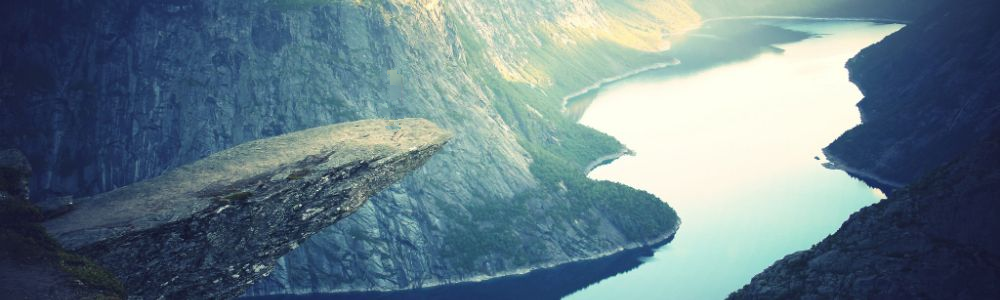
\includegraphics[width=0.4\textwidth]{figures/resultTroll9.png}}
%\caption{Suppression d'une personne au milieu d'un paysage}
%\end{figure}
\begin{figure}[H]
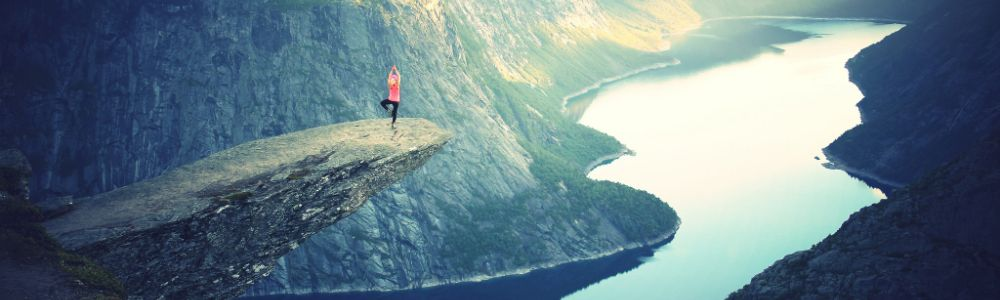
\includegraphics[width=0.5\textwidth]{figures/trolltunga.jpg}\label{fig:troll}
\end{figure}
\begin{figure}[H]
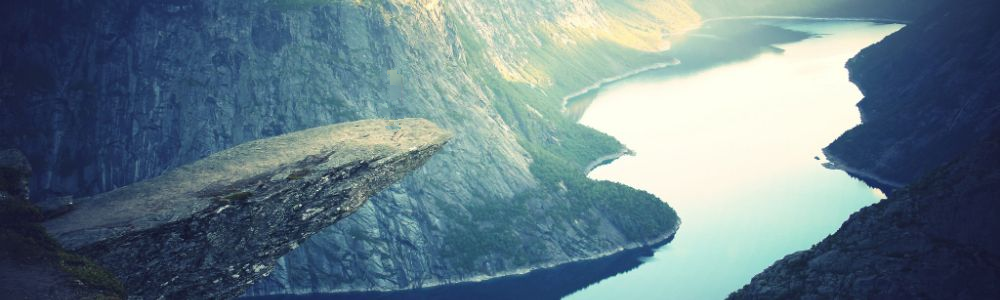
\includegraphics[width=0.5\textwidth]{figures/resultTroll9.png}\label{fig:trollb}
\caption{Suppression d'une personne au milieu d'un paysage}
\end{figure}


\end{block}

\end{column}


\end{columns}

\begin{columns}[t]
\begin{column}{.02\textwidth} \end{column}
\begin{column}{.930\textwidth} 
\begin{block}{\Large Discussion}
\begin{columns}[t]
\begin{column}{.496\textwidth}

\textbf{Résultats}
\begin{itemize}
\item Restauration correcte malgré quelques artefacts
\item Reconstruction inférieure en qualité vis à vis des attentes
\item Implémentation lente comparée au travail de Criminisi [3]
\end{itemize}
\textbf{Limitations}
\begin{itemize}
\item Importance de la \textbf{taille du patch} : trop grand (pixelise, ne capture pas toutes les variations), trop petit (ne capture pas corréctement les variations des textures plus grande). Doit être légèrement plus grand que le plus grand élément de texture. 
\item Echec de reconstruction sur \textbf{les bordures} de l'image
\item Lab : \textbf{SSD} sous norme CIE 74, échoue parfois à détecter un patch similaire
\end{itemize}


\begin{figure}[H]
\centering
\subfigure[Originale avec occlusion]{\label{fig:order} 
\includegraphics[width=0.3\textwidth]{figures/fillorderd.png}}
\subfigure[Inpainted]{ 
\includegraphics[width=0.3\textwidth]{figures/resultFillOrder35.png}}
\caption{Inpainting de test pour les structures linéaires, démontre l'importance de la taille du patch}
\end{figure}

\end{column}
\begin{column}{.496\textwidth} 
\textbf{Améliorations futures}
\begin{itemize}
\item SSD sous norme CIE 94 ou 2000 - prendre en compte l'uniformité perceptuelle
\item Patch de \textbf{taille variable} pour minimiser la distance à chaque application de texture
\item \textbf{Zone de recherche} du patch à identifier (pas dans toute l'image) - Gain de temps et éventuellement amélioration des résultats avec des patchs plus cohérent dans une région proche
\item Interface graphique pour masquage manuel 
\item Utilisation des \textbf{GraphCut} pour séléctionner la meilleure zone à applliquer lors de recouvrement de patch. 
\end{itemize}

\begin{figure}[H]
\centering
\subfigure[Originale]{\label{fig:lake} 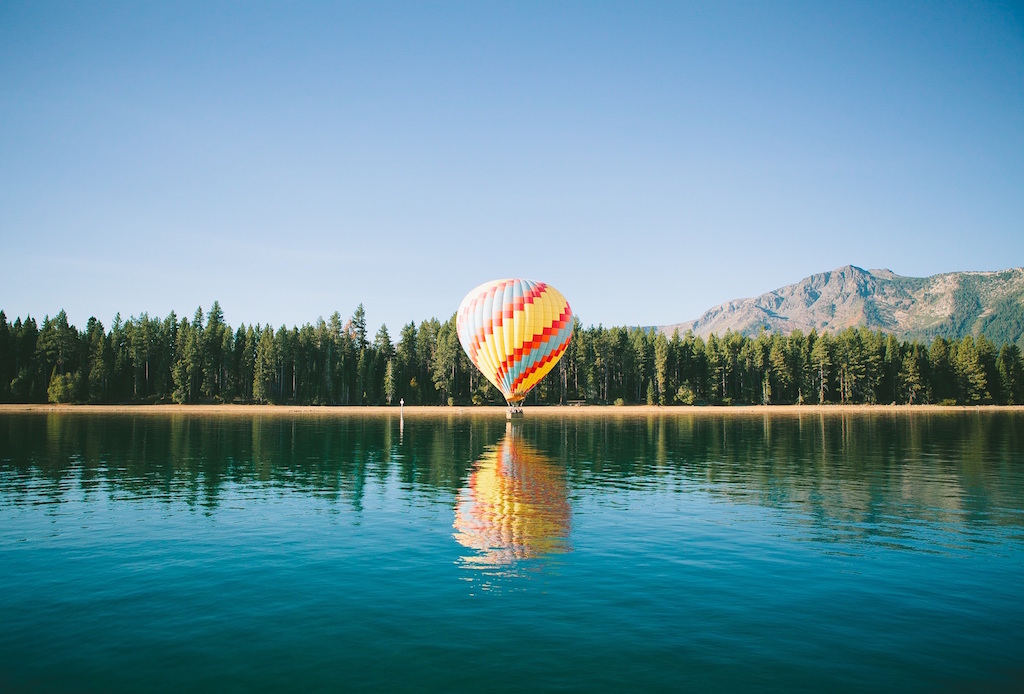
\includegraphics[width=0.24\textwidth]{figures/lakeandballoon.jpg}}
\subfigure[patch taille 5]{\label{fig:lakeb} 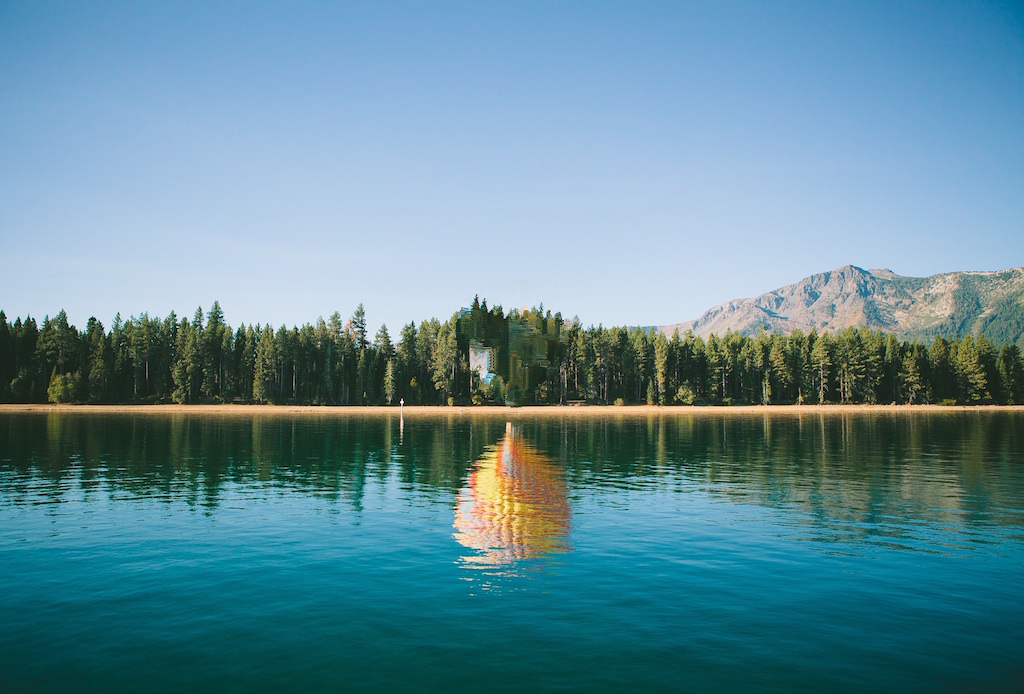
\includegraphics[width=0.24\textwidth]{figures/resultBallon5.png}}
\subfigure[patch taille 13]{\label{fig:lakec}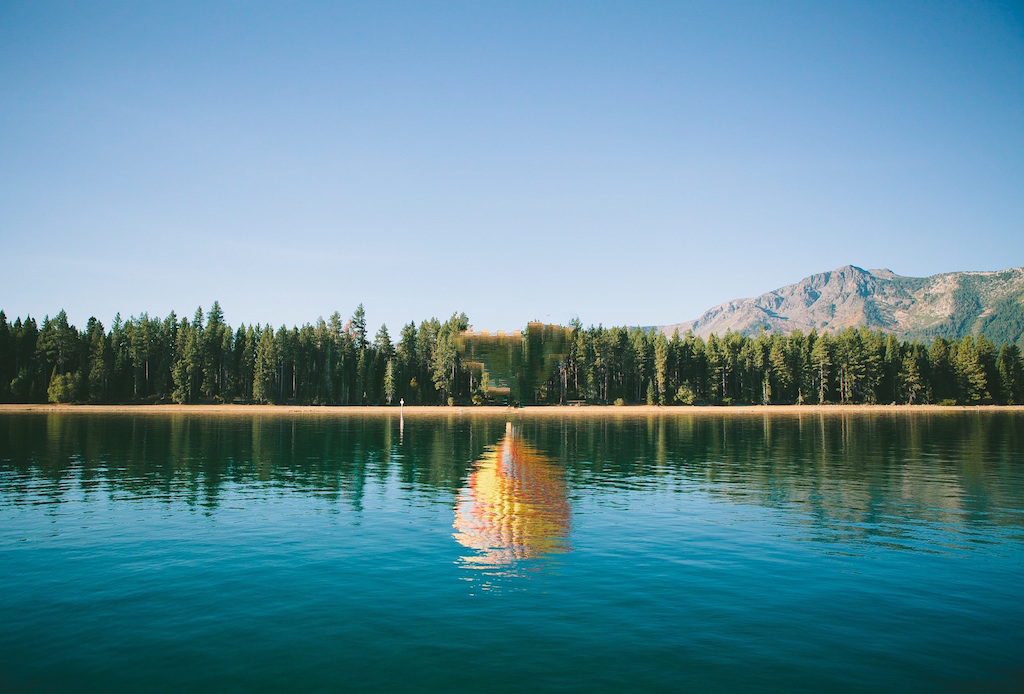
\includegraphics[width=0.24\textwidth]{figures/resultBallon13.png}}
\subfigure[patch 9 et masque complet]{\label{fig:laked}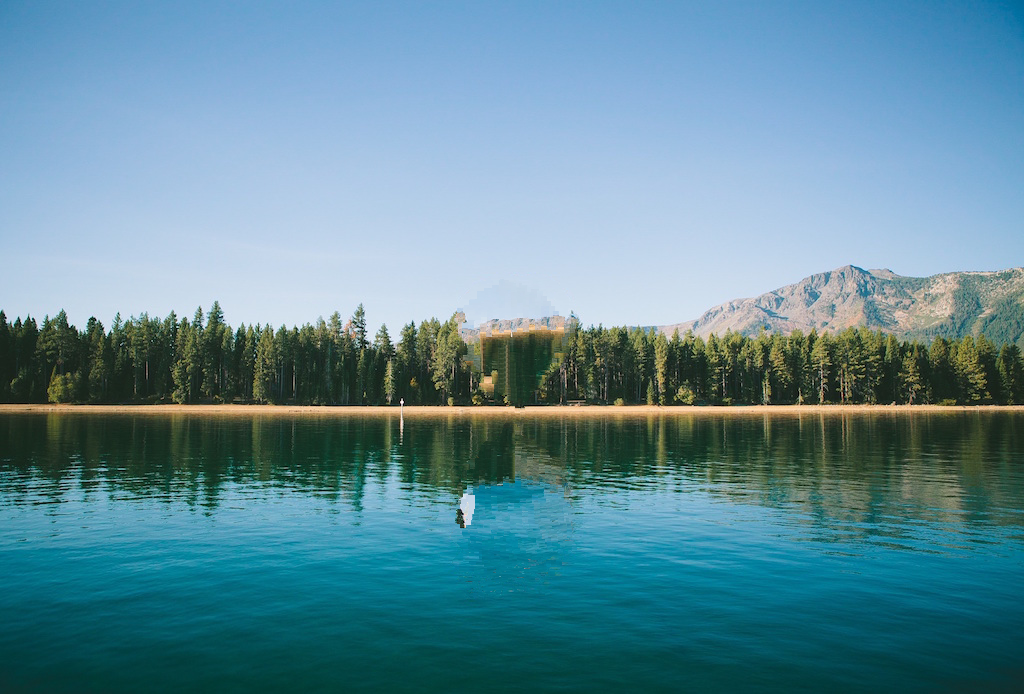
\includegraphics[width=0.24\textwidth]{figures/resultBallonLake9.png}}
\caption{Inpainting d'une montgolfière sur un Lac}
\end{figure}

\begin{block}{Références}
[1] Bertalmio et al, Image Inpainting. Proceedings of the 27th annual conference on Computer graphics and interactive techniques, 2000 \hfill \break 
[2] Bertalmio et al, Simultaneous structure and texture image inpainting, IEEE Transactions on image processing, 2003 \hfill \break
[3] Criminisi et al, Region filling and object removal by exemplar based image inpainting. IEEE Transactions on image processing, 2004 \hfill \break
[4] \alert TECHNIQUE ONLY TEXTURE SYNTHESIS

\end{block}
\end{column}
\end{columns}
\end{block}
\end{column}
\begin{column}{.02\textwidth} \end{column}
\end{columns}

\end{frame}
\bibliographystyle{\small}
\end{document}
